\documentclass[11pt]{article}
\usepackage[margin=1in]{geometry}
\usepackage{graphicx}
\usepackage{hyperref}
\usepackage{booktabs}
\usepackage{amsmath}
\usepackage{xcolor}

\newcommand{\todo}[1]{\textcolor{red}{\textbf{[TODO: #1]}}}

\title{Assignment 1: Opinion Network Formation}
\author{Team Name: Complex Network of Dynamic People}
\date{\today}

\begin{document}
\maketitle

% =====================================================================
\section*{GitHub Link to Code}
\url{https://github.com/ShreeLite/DPCN_A1}

% =====================================================================
\section{Dataset Documentation}
\label{sec:dataset}

The data cleaning and encoding pipeline described below was implemented
as part of the network construction workstream (see \texttt{build\_network.py});
this section documents and elaborates on that process.

The raw survey collected responses from 96 students across 60 statements
on a 5-point Likert scale (Strongly Disagree, Disagree, Neutral, Agree,
Strongly Agree), evenly split into four topics of 15 items each:
Technology (prefix \texttt{T}), Education (\texttt{E}), Ethics/Society
(\texttt{S}), and Environment (\texttt{V}). Before any analysis, the raw
responses were cleaned in two stages. First, the string ``No Comments''
was treated as a genuinely missing response rather than a neutral
(``Neutral'') opinion, since a respondent skipping a question and a
respondent actively choosing the midpoint of the scale are not the same
thing. Second, respondents who left more than 50\% of the 60 items blank
were removed entirely (9 of the original 96 respondents), since a
profile that is mostly missing cannot be meaningfully placed in an
opinion network -- this left 87 usable respondents. Any remaining sparse
gaps (a respondent missing a handful, but not most, of the items) were
filled with that item's class-average response, a conservative choice
that avoids manufacturing an artificially strong opinion where none was
expressed. Finally, the ordinal Likert scale was encoded numerically as
Strongly Disagree $=-2$, Disagree $=-1$, Neutral $=0$, Agree $=+1$,
Strongly Agree $=+2$, producing the $87 \times 60$ numeric matrix
(\texttt{outputs/encoded\_responses.csv}) that both the person-opinion
and item-opinion networks in this report are built from.

\subsection*{Descriptive Statistics and Data Exploration}

To understand what the cleaned data actually looks like before any
network is built, Table~\ref{tab:topic_stats} summarizes the encoded
response distribution for each of the four topics (pooling all 87
respondents $\times$ 15 items per topic).

\begin{table}[h]
\centering
\begin{tabular}{lrrrrr}
\toprule
Topic & Mean & Std.\ Dev. & Median & \% Agree+ & \% Disagree- \\
\midrule
Environment     & 1.39 & 0.75 & 2 & 89.7\% & 2.3\%  \\
Ethics/Society  & 1.28 & 0.83 & 1 & 86.1\% & 3.7\%  \\
Technology      & 1.00 & 0.99 & 1 & 74.7\% & 8.2\%  \\
Education       & 0.91 & 1.15 & 1 & 70.4\% & 13.7\% \\
\bottomrule
\end{tabular}
\caption{Per-topic descriptive statistics of the encoded response
matrix ($-2$ = Strongly Disagree, $+2$ = Strongly Agree). ``\% Agree+''
and ``\% Disagree$-$'' give the share of all (respondent, item) values
in that topic that were Agree/Strongly Agree or Disagree/Strongly
Disagree respectively.}
\label{tab:topic_stats}
\end{table}

\begin{figure}[h]
\centering
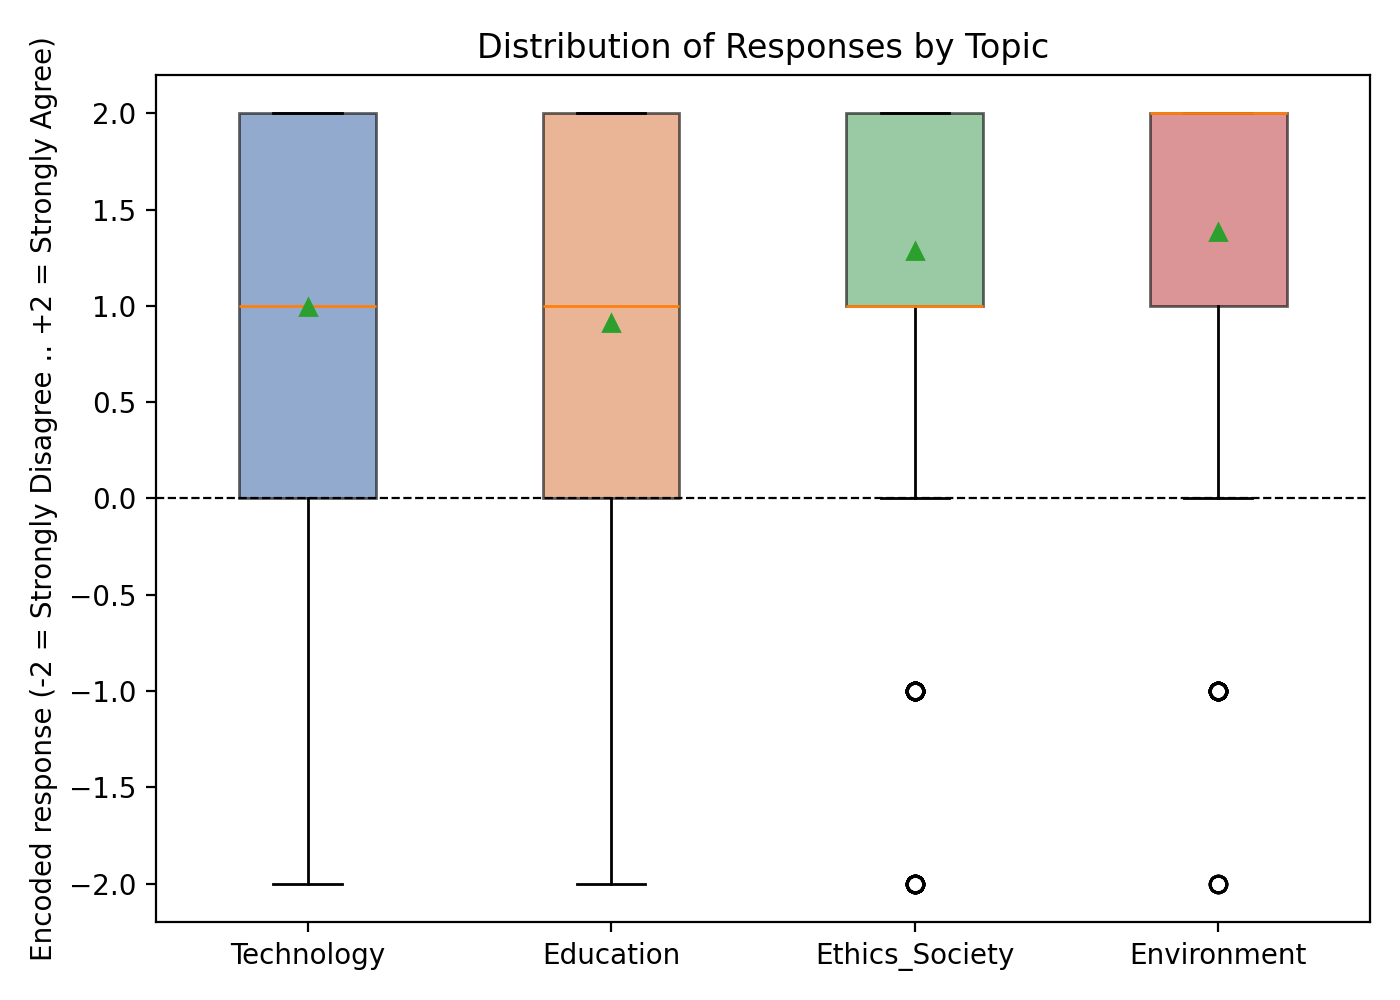
\includegraphics[width=0.65\textwidth]{../../dataset_documentation/figures/topic_response_boxplot.png}
\caption{Distribution of encoded responses by topic. All four topics
skew positive; Education has the widest spread and the only topic
whose interquartile range dips to Neutral.}
\label{fig:topic_boxplot}
\end{figure}

\begin{figure}[h]
\centering
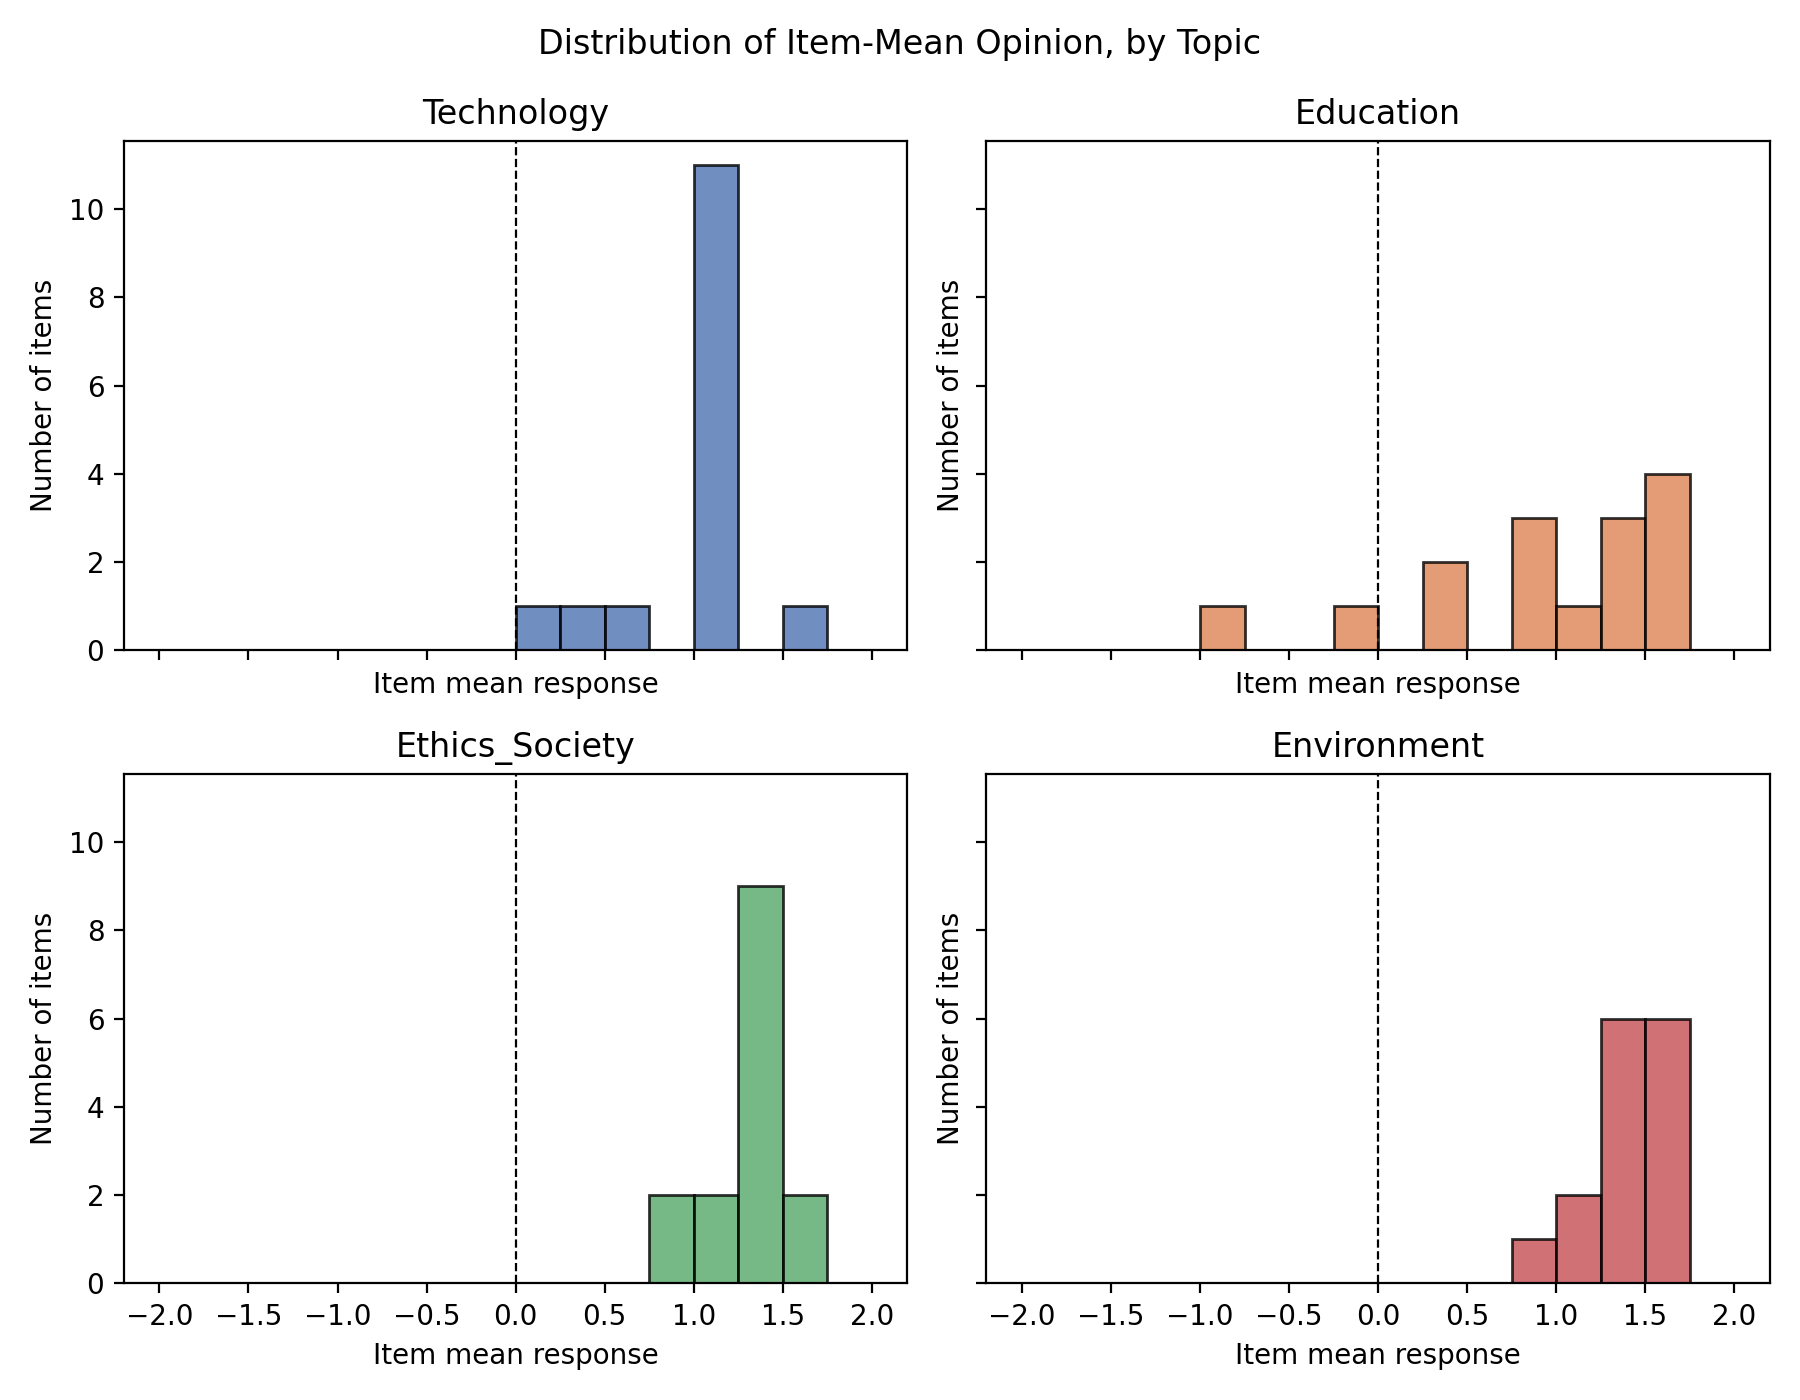
\includegraphics[width=0.85\textwidth]{../../dataset_documentation/figures/item_mean_distribution.png}
\caption{Distribution of per-item mean opinion (60 items total),
faceted by topic. Technology and Environment items are tightly
concentrated around a single positive mean; Education items are the
most dispersed, including the only two topic-level items with a
negative mean.}
\label{fig:item_mean_dist}
\end{figure}

Every topic has a positive mean, i.e.\ the class leans toward agreement
on nearly every statement, but the four topics are not equally
consensual. Environment and Ethics/Society have both the highest means
\emph{and} the lowest standard deviations -- around 88\% of all
responses to these items are Agree or Strongly Agree, and almost nobody
disagrees. Education has the lowest mean and by far the highest spread
(std.\ 1.15): the most contested individual items in the entire survey
are all Education items concerning assessment and attendance policy
(e.g.\ ``class attendance should be compulsory'', ``online learning can
effectively complement classroom teaching''), where personal experience
plausibly differs far more between students than it does for abstract
ethics or environment statements. The most consensual items, by
contrast, are broad normative statements (e.g.\ ``continuous learning
and skill development are essential'', ``companies should be held
accountable for the environmental impacts of their activities'') that a
Likert survey rarely gets genuine disagreement on.

\paragraph{A note on self-report survey bias.} This skew toward
agreement is exactly what we would expect if several well-known biases
in self-report surveys are present here. \textbf{Social desirability
bias} means respondents tend to agree with statements framed as
normatively ``good'' positions -- sustainability, ethics, personal
responsibility -- regardless of their private attitude, particularly in
a class survey where responses are not fully anonymous to the
respondent's peer group. \textbf{Acquiescence bias} (a general tendency
to agree with whatever is presented) would independently push every
topic's mean upward, and is consistent with the fact that even the
least-agreed-with topic (Education) still has a positive mean.
\textbf{Self-selection} in who chose to complete the survey at all may
also matter: 9 of 96 respondents were dropped for leaving over half the
survey blank, and the remaining 87 who engaged with all 60 statements
may be more opinionated or more agreeable than a true random sample of
the class. Because of this skew, raw agreement levels should be read
with caution, and the \emph{relative} structure captured by
correlation-based similarity -- used throughout both the person-opinion
network (Section~\ref{sec:pipeline}) and the item-opinion network
(Section~\ref{sec:item_network}) -- is a more robust signal of real
opinion differences than absolute response levels are.

% =====================================================================
\section{Pipeline Followed}
\label{sec:pipeline}

This section describes how the raw survey responses were transformed into
an opinion network.

\subsection{Data Cleaning and Encoding}
Respondents who left more than 50\% of the survey unanswered were removed
(9 of 96 respondents), leaving 87 usable respondents. The string
``No Comments'' was treated as a missing value rather than a neutral
opinion. Likert responses were mapped to an ordinal numeric scale from
$-2$ (Strongly Disagree) to $+2$ (Strongly Agree), and any remaining
sparse gaps were filled with that item's class-average response.

\subsection{Similarity Measure}
Pairwise opinion similarity between respondents was computed using the
\textbf{Pearson correlation coefficient} across their answer vectors,
rather than cosine similarity or Euclidean distance. Correlation was
chosen because it captures whether two respondents' opinions rise and
fall \emph{together} across statements, and is invariant to a
respondent's individual tendency to answer more or less extremely
overall -- a scale bias rather than a genuine opinion difference.

\subsection{Graph Construction}
The dense $87 \times 87$ similarity matrix was sparsified using
\textbf{mutual $k$-Nearest-Neighbours} with $k=8$: an edge between
respondents $i$ and $j$ was retained only if each was among the other's
top-8 most similar peers. This produces a graph reflecting genuinely
reciprocal opinion closeness, avoids an uninformative fully-connected
graph, and sidesteps the need to hand-tune a similarity threshold.

In addition to the overall network (built from all 60 items), four
topic-specific sub-networks were constructed using the same procedure
restricted to each topic's 15 items, to allow cross-topic comparison
of clustering structure.

\subsection{Community Detection}
Louvain modularity maximization was applied to the overall network to
identify opinion communities. The same procedure was applied
independently to each topic sub-network for comparison.

\todo{PRATHISH (Statistical Validation): briefly describe your null-model validation
methodology here (1 short paragraph) -- e.g. ``To assess whether the
observed community structure is statistically meaningful, modularity
was compared against a null distribution generated from N random graphs
matched on node count, edge count, and degree sequence...''}

\subsection{Item-Opinion Network Construction}
\label{sec:item_network}
In addition to the person-opinion network above, a second network was
built with the opposite orientation: nodes are the 60 survey
\emph{items} rather than the 87 respondents, and an edge reflects
whether two items were answered similarly across respondents --
i.e., whether people who agreed strongly with one statement also
tended to agree strongly with the other. This is the exact transpose of
the person-network pipeline: Pearson correlation was computed between
every pair of items' 87-respondent answer vectors (rather than between
respondents' 60-item vectors), and the resulting $60\times 60$
correlation matrix was sparsified with the same mutual $k$-Nearest-Neighbours
procedure ($k=8$) used for the person network, for direct methodological
comparability. Louvain community detection was then applied to the
resulting item network, and the discovered communities were compared
against the survey's own four a-priori topic labels using Adjusted Rand
Index, to test whether real opinion structure follows the survey's
topic design or cuts across it.

% =====================================================================
\section{Analysis and Visualizations}
\label{sec:analysis}

\subsection{Overall Network Structure}

\begin{table}[h]
\centering
\begin{tabular}{lr}
\toprule
Metric & Value \\
\midrule
Nodes & 87 \\
Edges & 134 \\
Density & 0.036 \\
Average clustering coefficient & 0.157 \\
Average path length (largest component) & 3.86 \\
Diameter (largest component) & 9 \\
Number of connected components & 18 \\
Largest component size & 66 \\
Number of Louvain communities & 25 \\
Modularity & 0.578 \\
\bottomrule
\end{tabular}
\caption{Overall opinion network metrics.}
\label{tab:overall_metrics}
\end{table}

\begin{figure}[h]
\centering
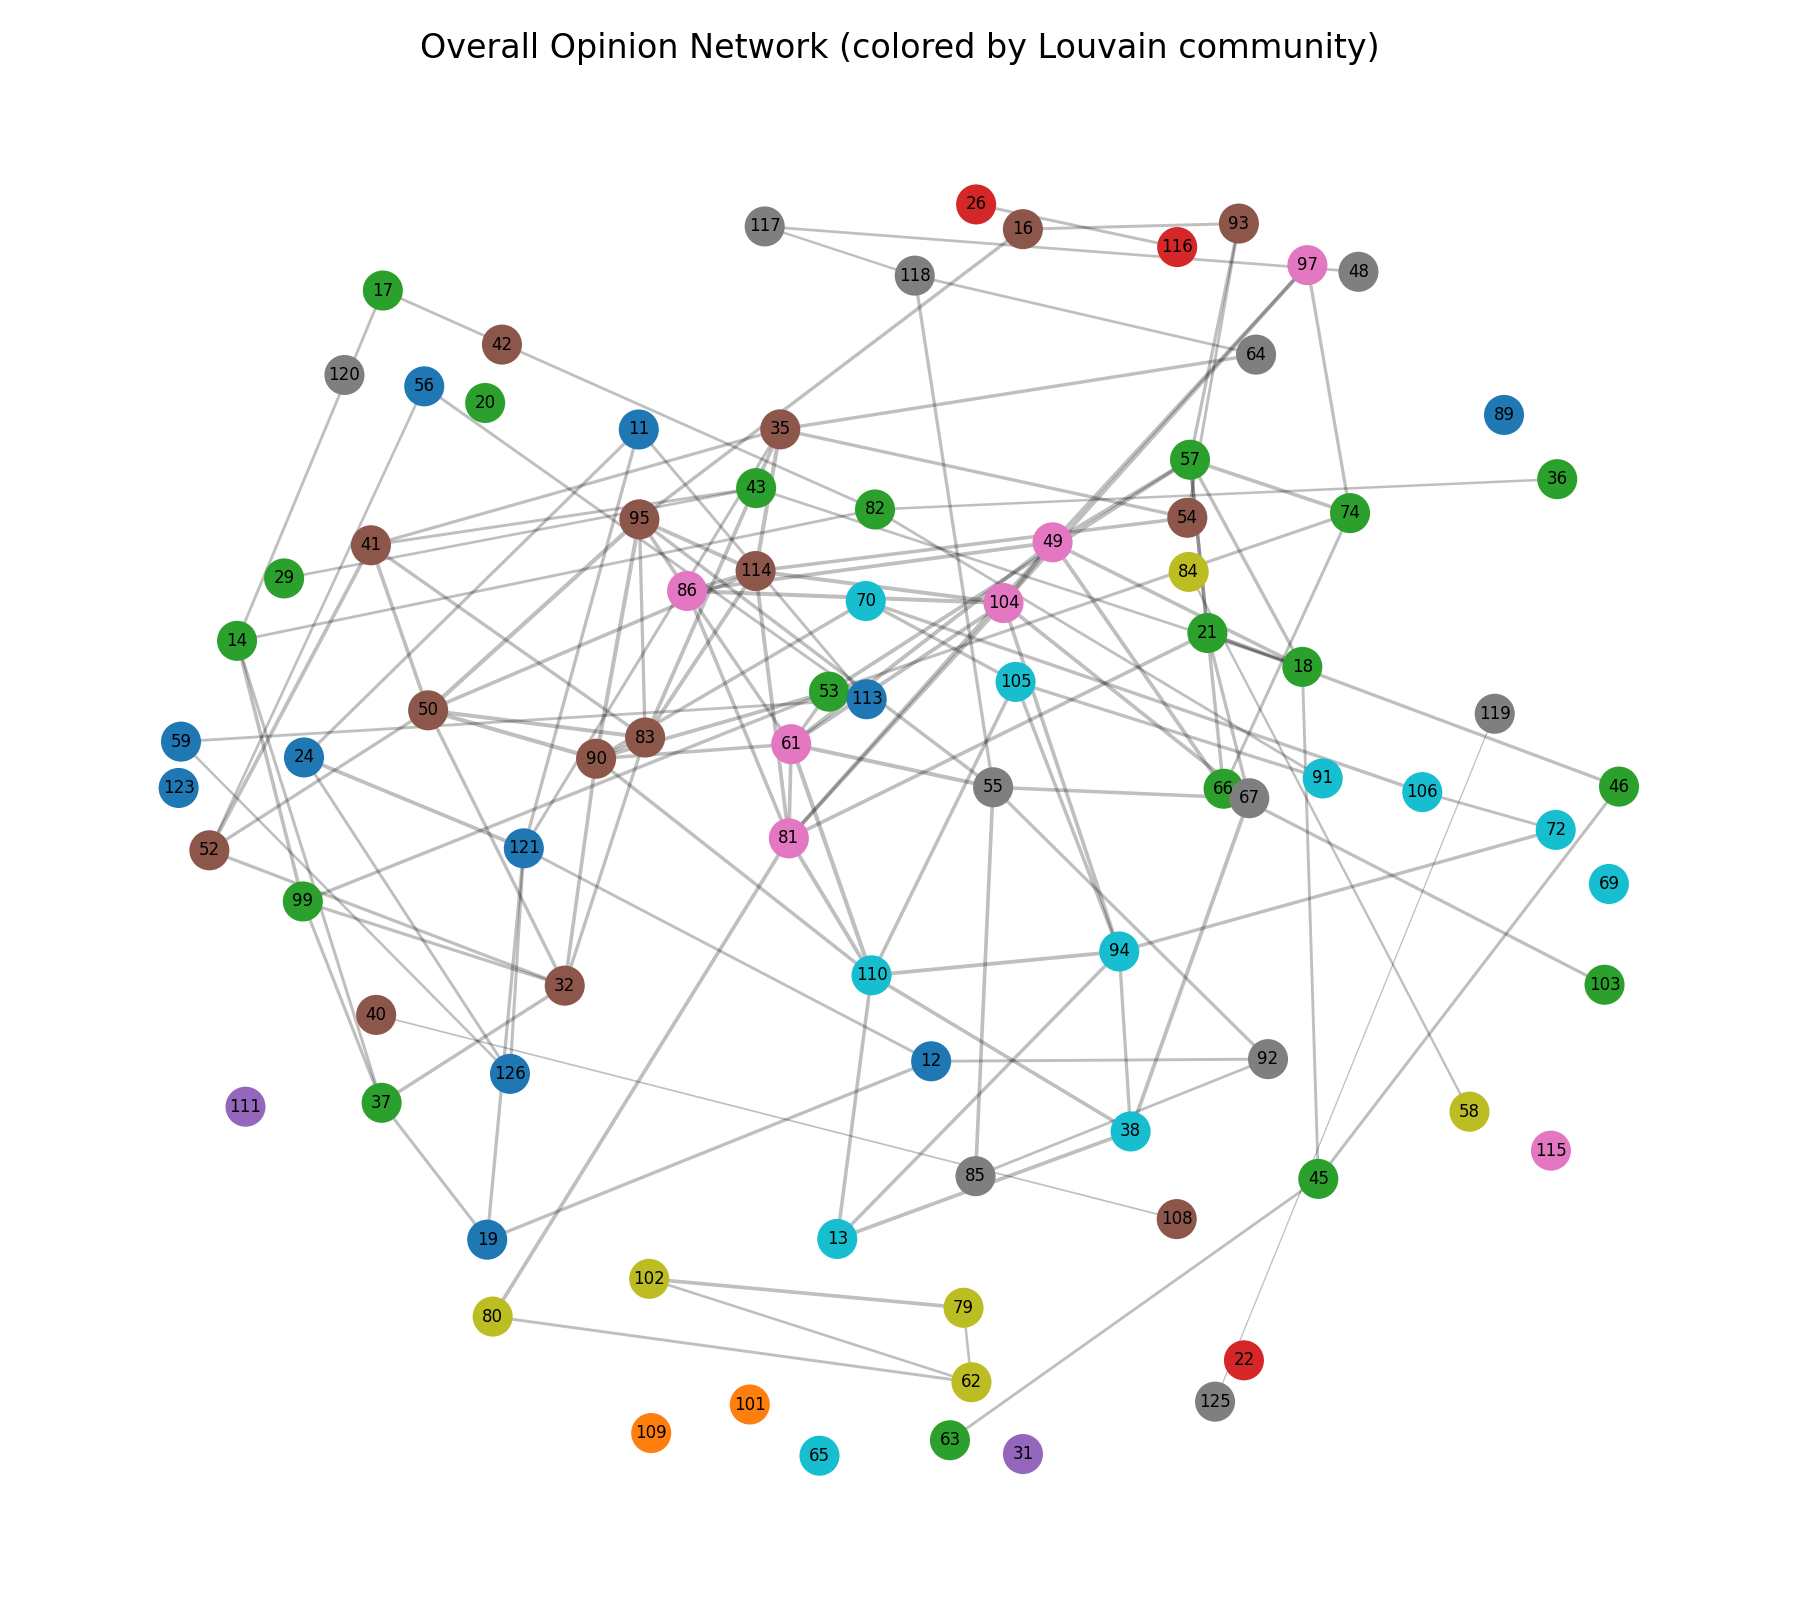
\includegraphics[width=0.75\textwidth]{../figures/overall_network.png}
\caption{Overall opinion network, nodes colored by Louvain community.}
\label{fig:overall_network}
\end{figure}

\begin{figure}[h]
\centering
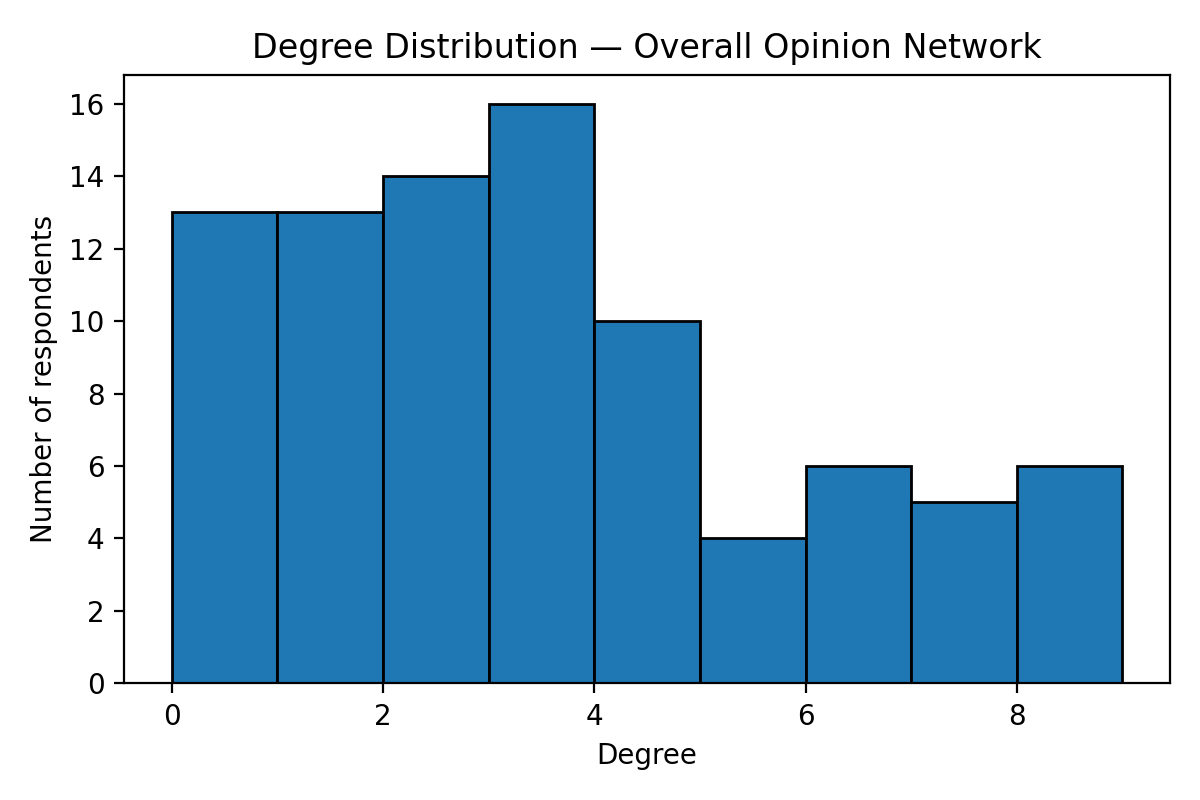
\includegraphics[width=0.6\textwidth]{../figures/degree_distribution.png}
\caption{Degree distribution of the overall opinion network.}
\label{fig:degree_dist}
\end{figure}

\subsection{Topic Sub-Networks and Cross-Topic Comparison}

Table~\ref{tab:topic_metrics} summarizes the four topic-specific
sub-networks.

\begin{table}[h]
\centering
\begin{tabular}{lrrr}
\toprule
Topic & Edges & Density \\
\midrule
Technology & 201 & 0.054 \\
Education & 176 & 0.047 \\
Ethics/Society & 227 & 0.061 \\
Environment & 193 & 0.052 \\
\bottomrule
\end{tabular}
\caption{Topic sub-network metrics (87 nodes each).}
\label{tab:topic_metrics}
\end{table}

\begin{figure}[h]
\centering
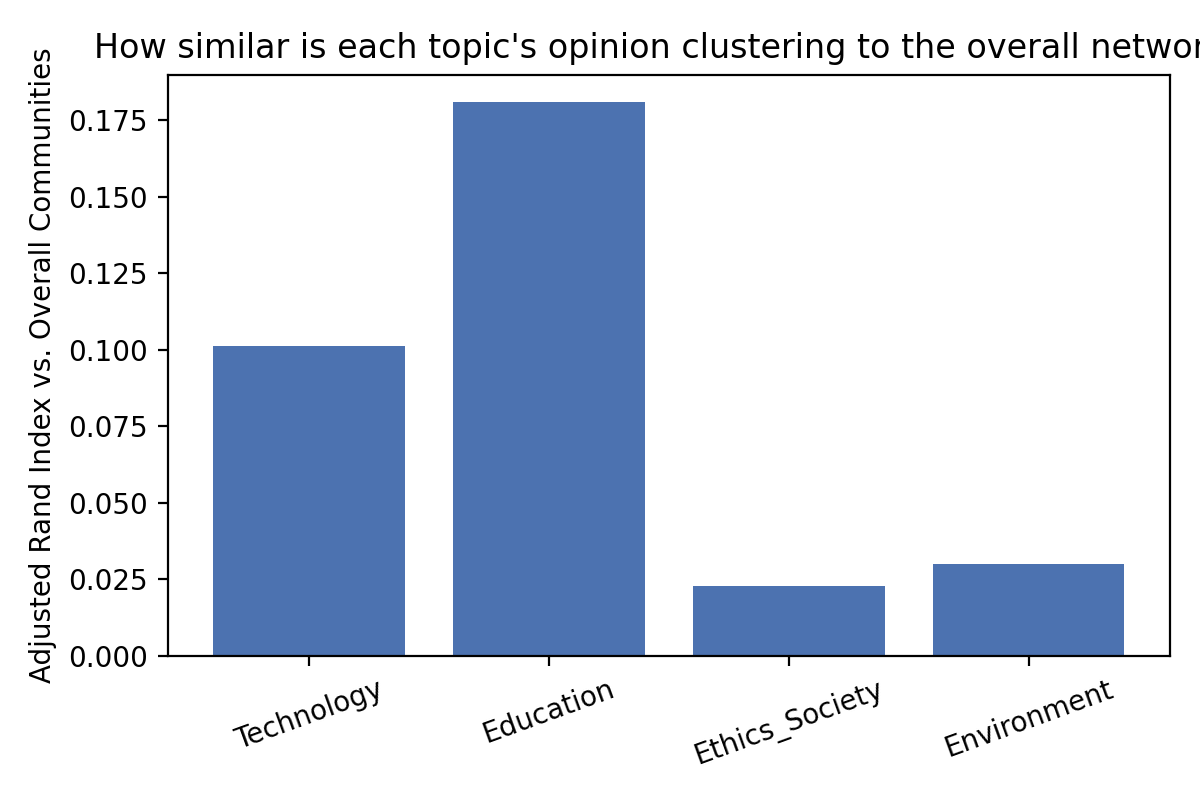
\includegraphics[width=0.6\textwidth]{../figures/cross_topic_ari.png}
\caption{Adjusted Rand Index between each topic's community structure
and the overall network's community structure.}
\label{fig:ari}
\end{figure}

\subsection{Opinion Bridges}

To identify respondents who structurally connect otherwise separate
opinion communities, betweenness centrality was computed for every node,
and the community diversity of each top-scoring node's immediate
neighborhood was examined (Table~\ref{tab:bridges}).

\begin{table}[h]
\centering
\begin{tabular}{lrrr}
\toprule
Respondent & Betweenness Centrality & Own Community & Neighbor Communities Spanned \\
\midrule
81 & 0.083 & 16 & 5 \\
35 & 0.090 & 12 & 3 \\
90 & 0.062 & 12 & 4 \\
55 & 0.074 & 18 & 3 \\
121 & 0.083 & 0 & 2 \\
\bottomrule
\end{tabular}
\caption{Top opinion-bridge respondents by betweenness centrality.}
\label{tab:bridges}
\end{table}

\begin{figure}[h]
\centering
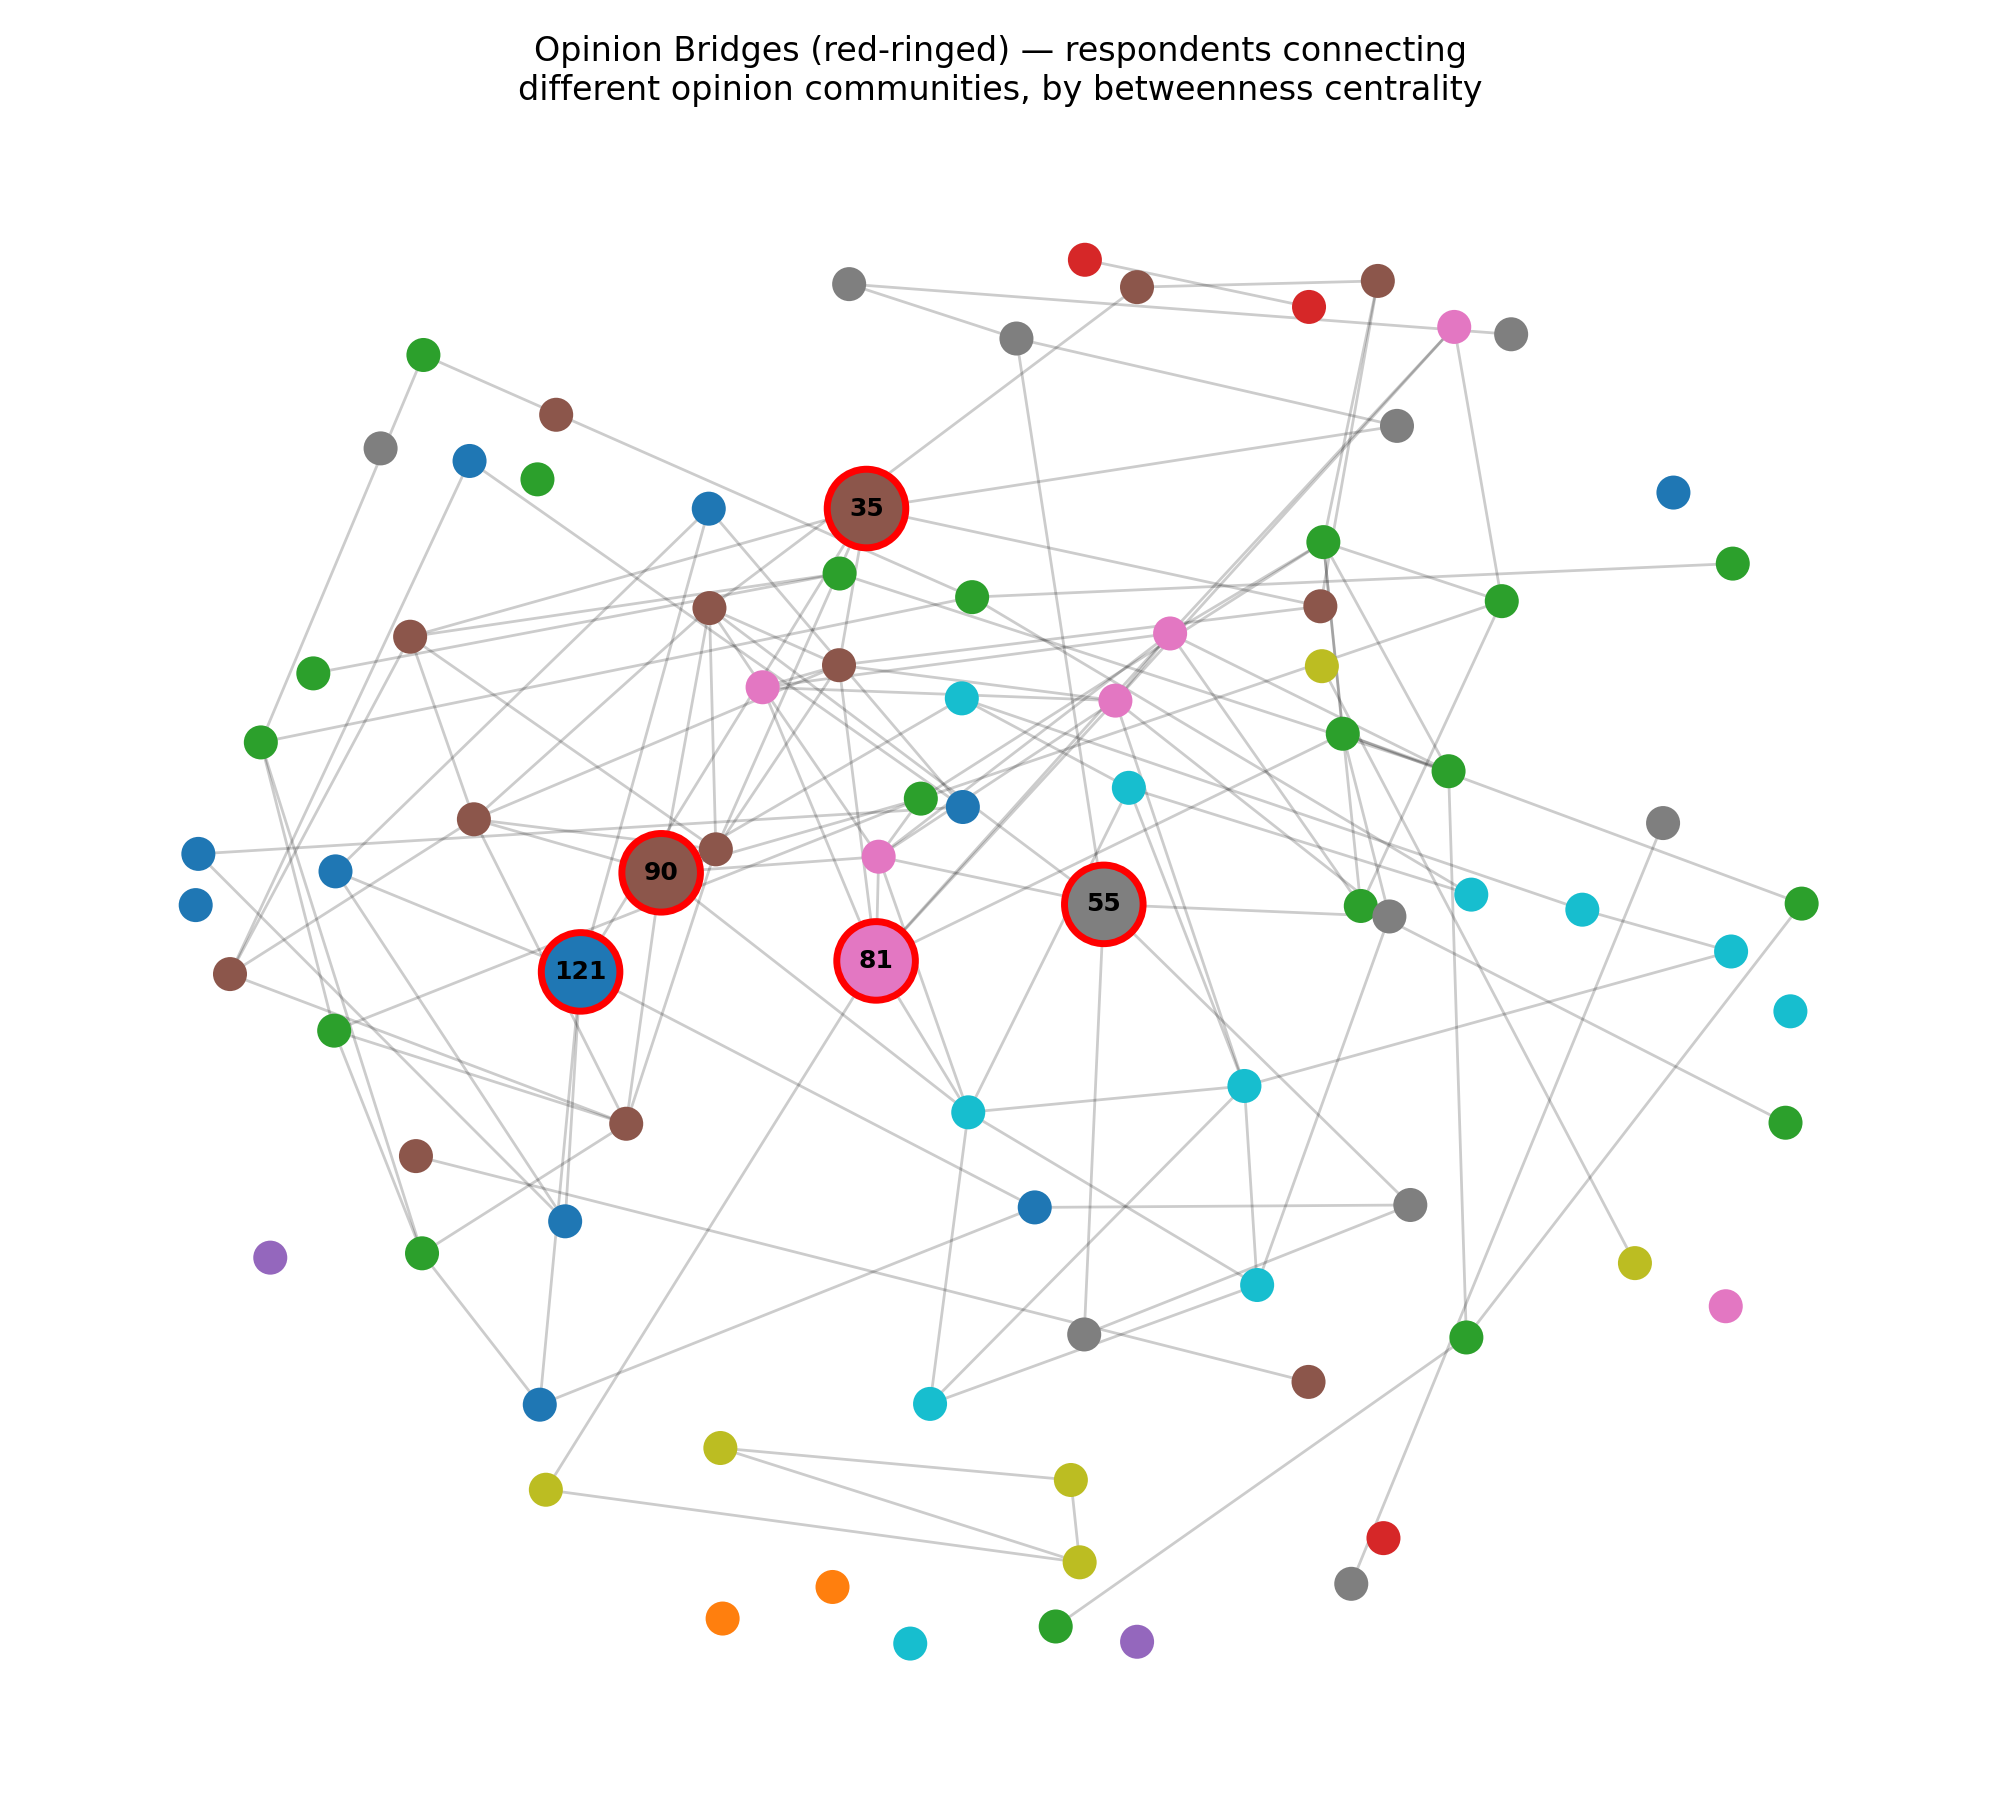
\includegraphics[width=0.75\textwidth]{../figures/opinion_bridges.png}
\caption{Opinion bridges (red-ringed nodes) overlaid on the overall network.}
\label{fig:bridges}
\end{figure}

\subsection{Community Opinion Archetypes}

For every community with at least 4 members, the average deviation from
the class-wide opinion score was computed per topic, producing
interpretable ``opinion archetypes'' for each cluster
(Figure~\ref{fig:archetypes}).

\begin{figure}[h]
\centering
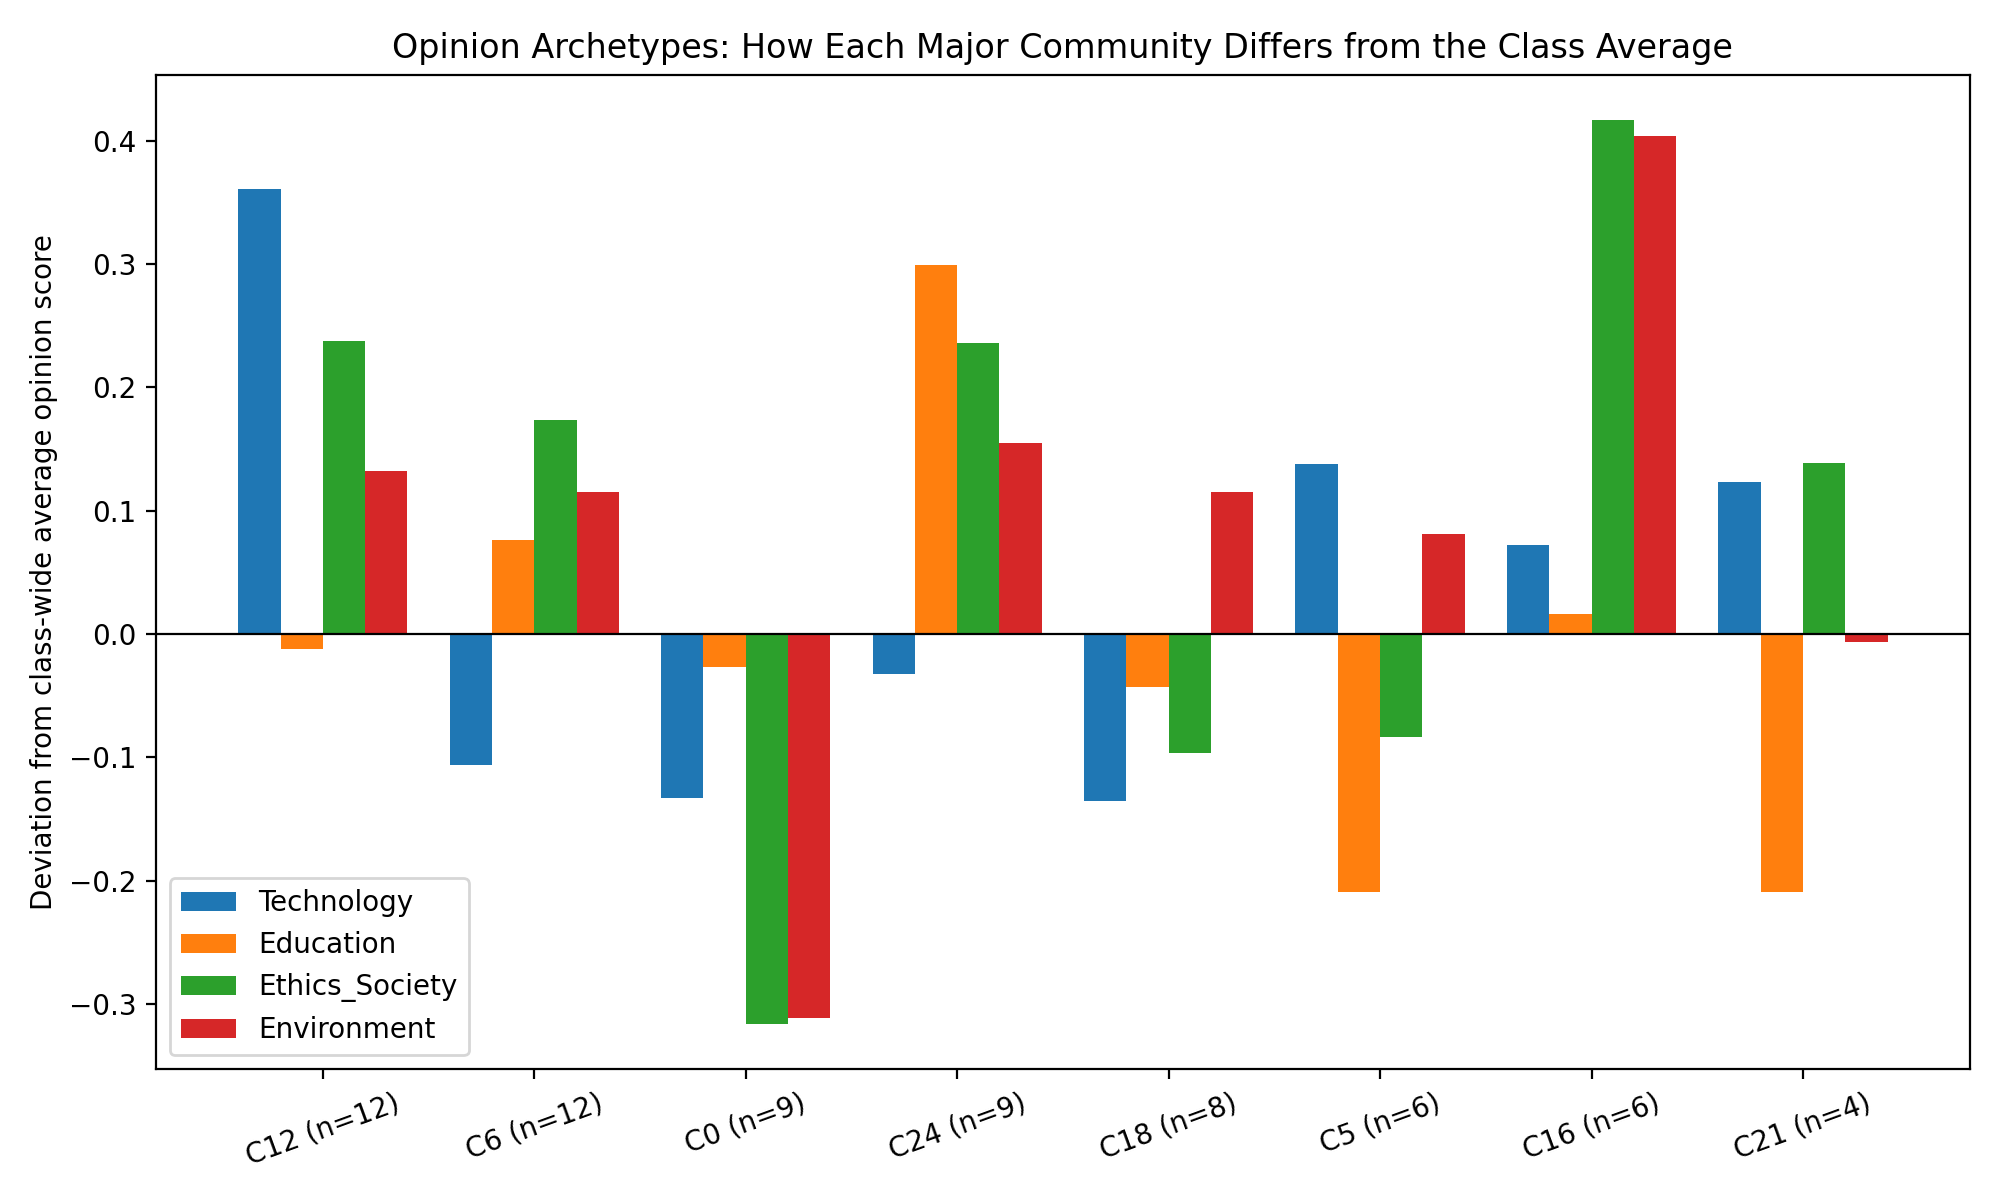
\includegraphics[width=0.85\textwidth]{../figures/community_opinion_profiles.png}
\caption{Opinion archetypes: deviation of each major community from the
class-wide average, by topic.}
\label{fig:archetypes}
\end{figure}

\subsection{Item-Opinion Network}
\label{sec:item_analysis}

Table~\ref{tab:item_metrics} summarizes the item-opinion network
constructed in Section~\ref{sec:item_network}.

\begin{table}[h]
\centering
\begin{tabular}{lr}
\toprule
Metric & Value \\
\midrule
Nodes (survey items) & 60 \\
Edges & 140 \\
Density & 0.079 \\
Average clustering coefficient & 0.107 \\
Average path length (largest component) & 3.04 \\
Diameter (largest component) & 7 \\
Number of connected components & 4 \\
Largest component size & 57 \\
Number of Louvain communities & 9 \\
Modularity & 0.428 \\
ARI vs.\ a-priori survey topics & 0.143 \\
\bottomrule
\end{tabular}
\caption{Item-opinion network metrics.}
\label{tab:item_metrics}
\end{table}

\begin{figure}[h]
\centering
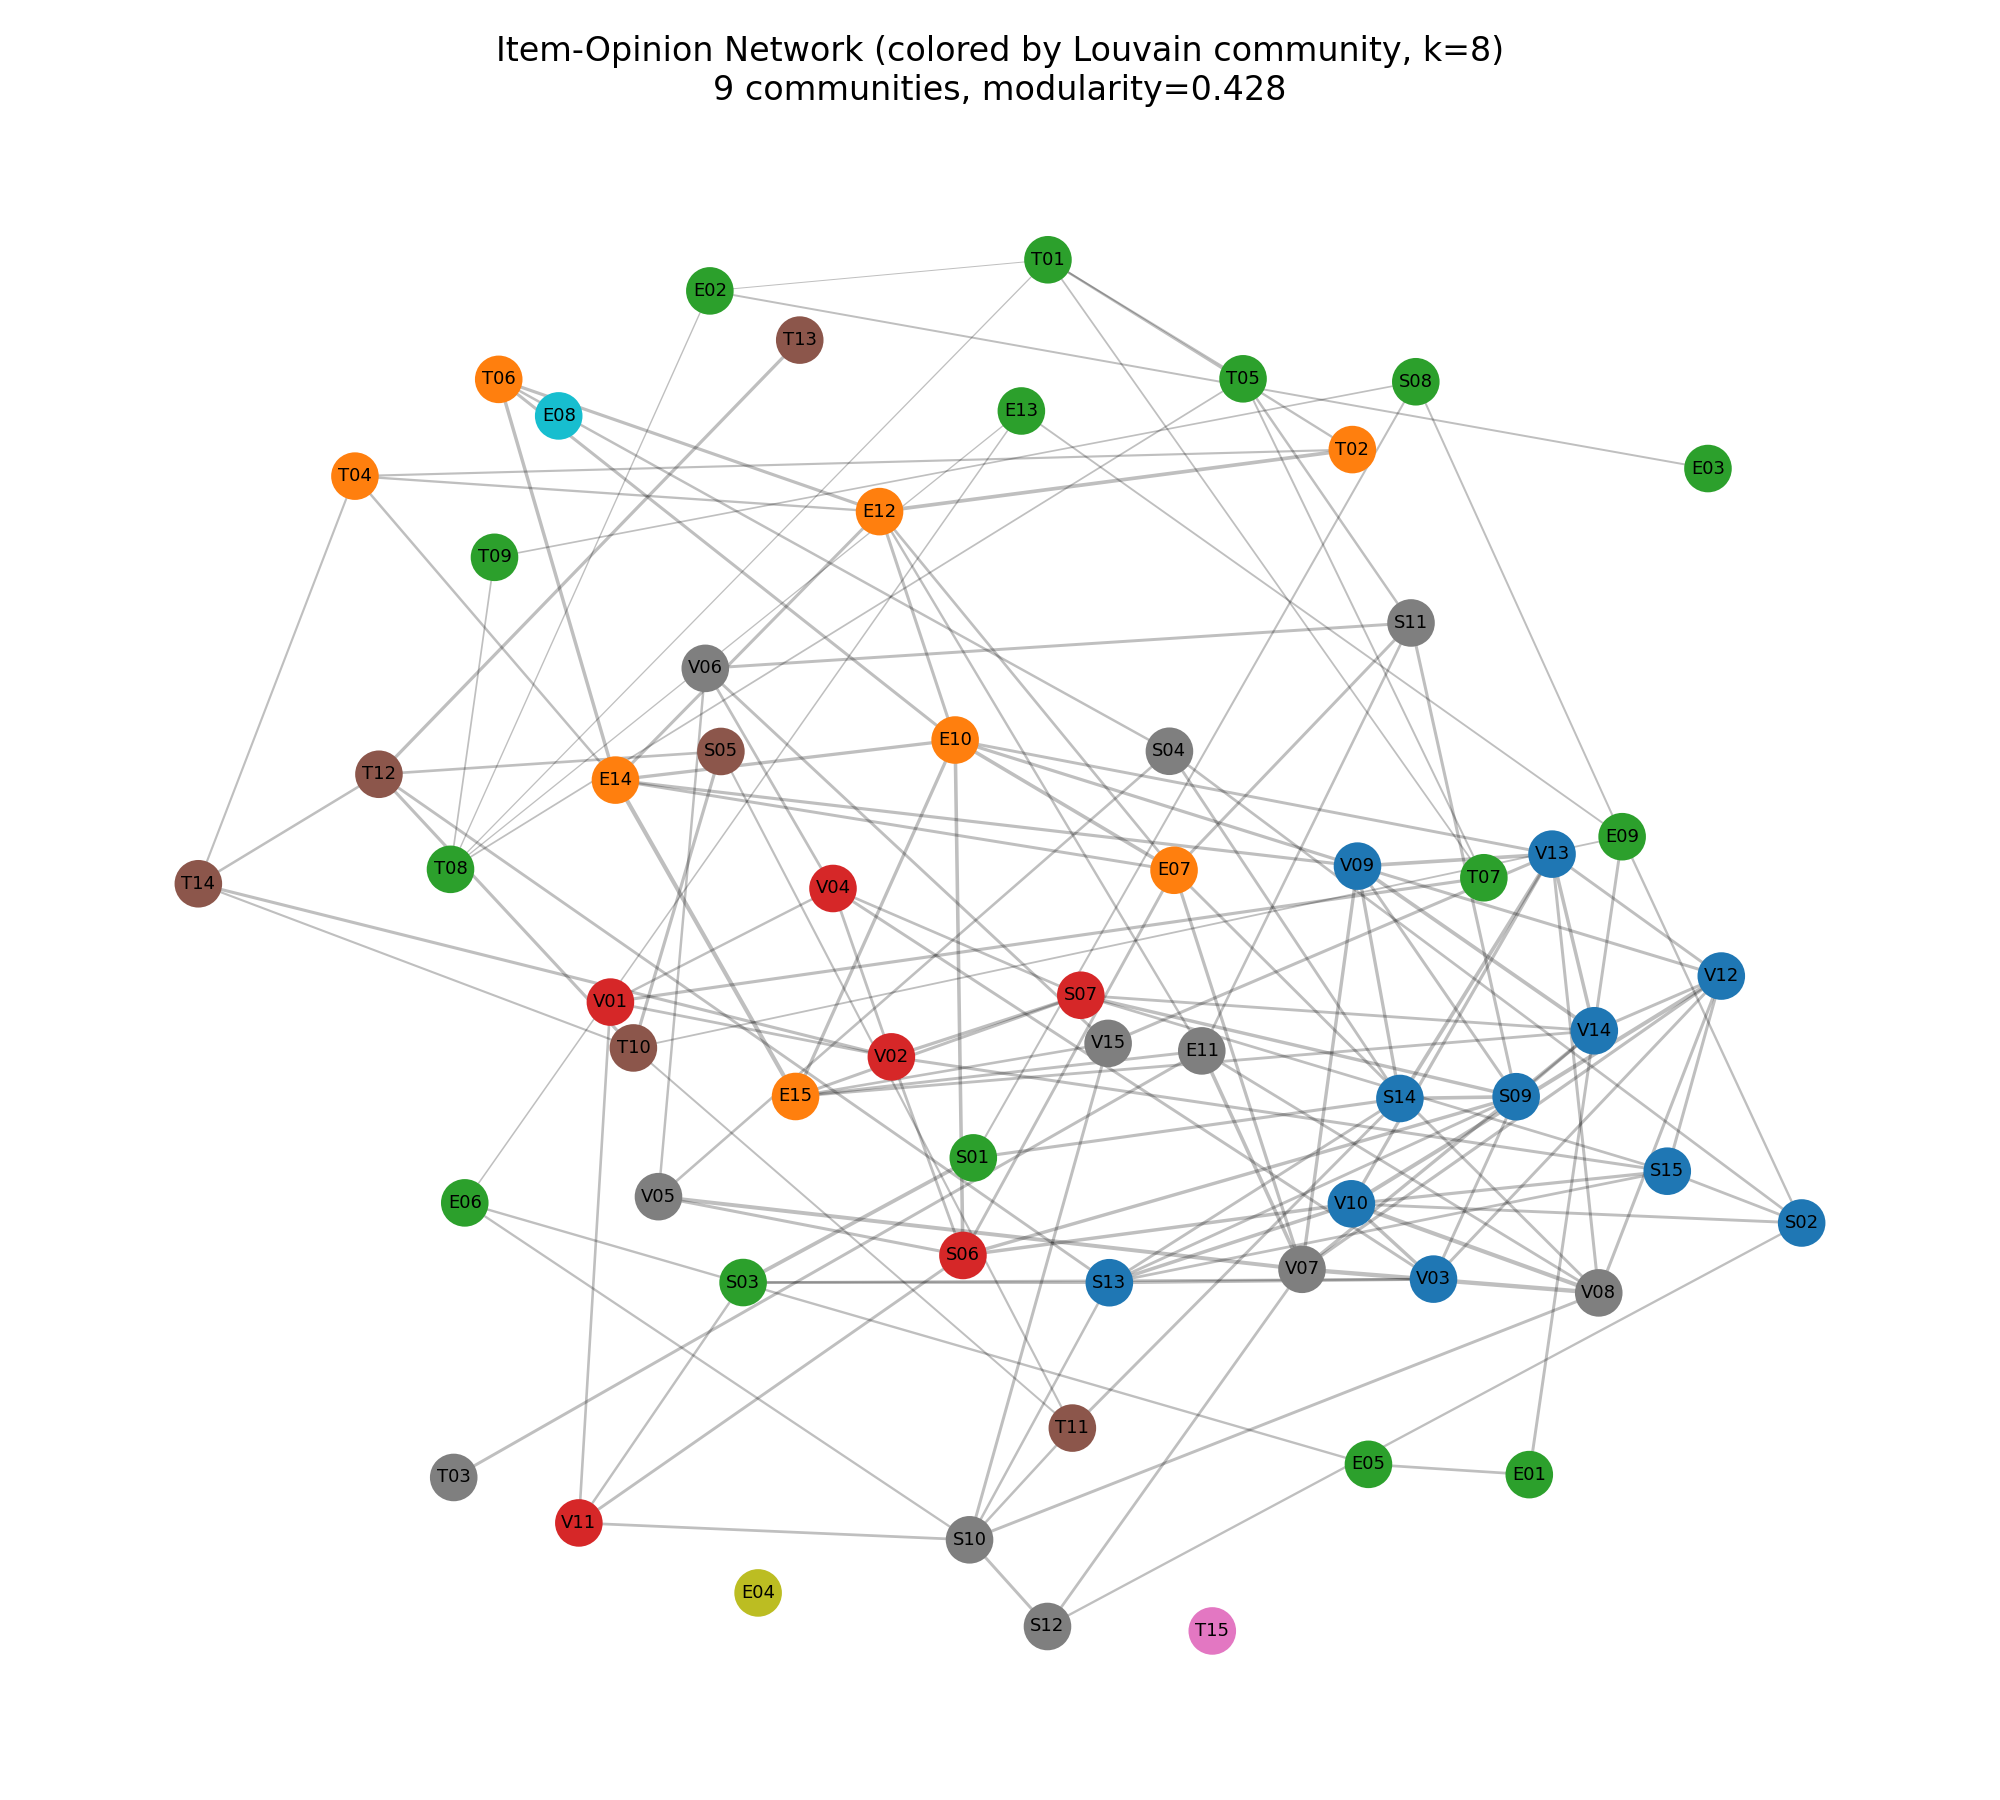
\includegraphics[width=0.75\textwidth]{../../item_network/figures/item_network_by_community.png}
\caption{Item-opinion network, nodes colored by Louvain community and
labeled by item code (e.g.\ T01 = Technology item 1). Node layout is
identical to Figure~\ref{fig:item_by_topic}.}
\label{fig:item_by_community}
\end{figure}

\begin{figure}[h]
\centering
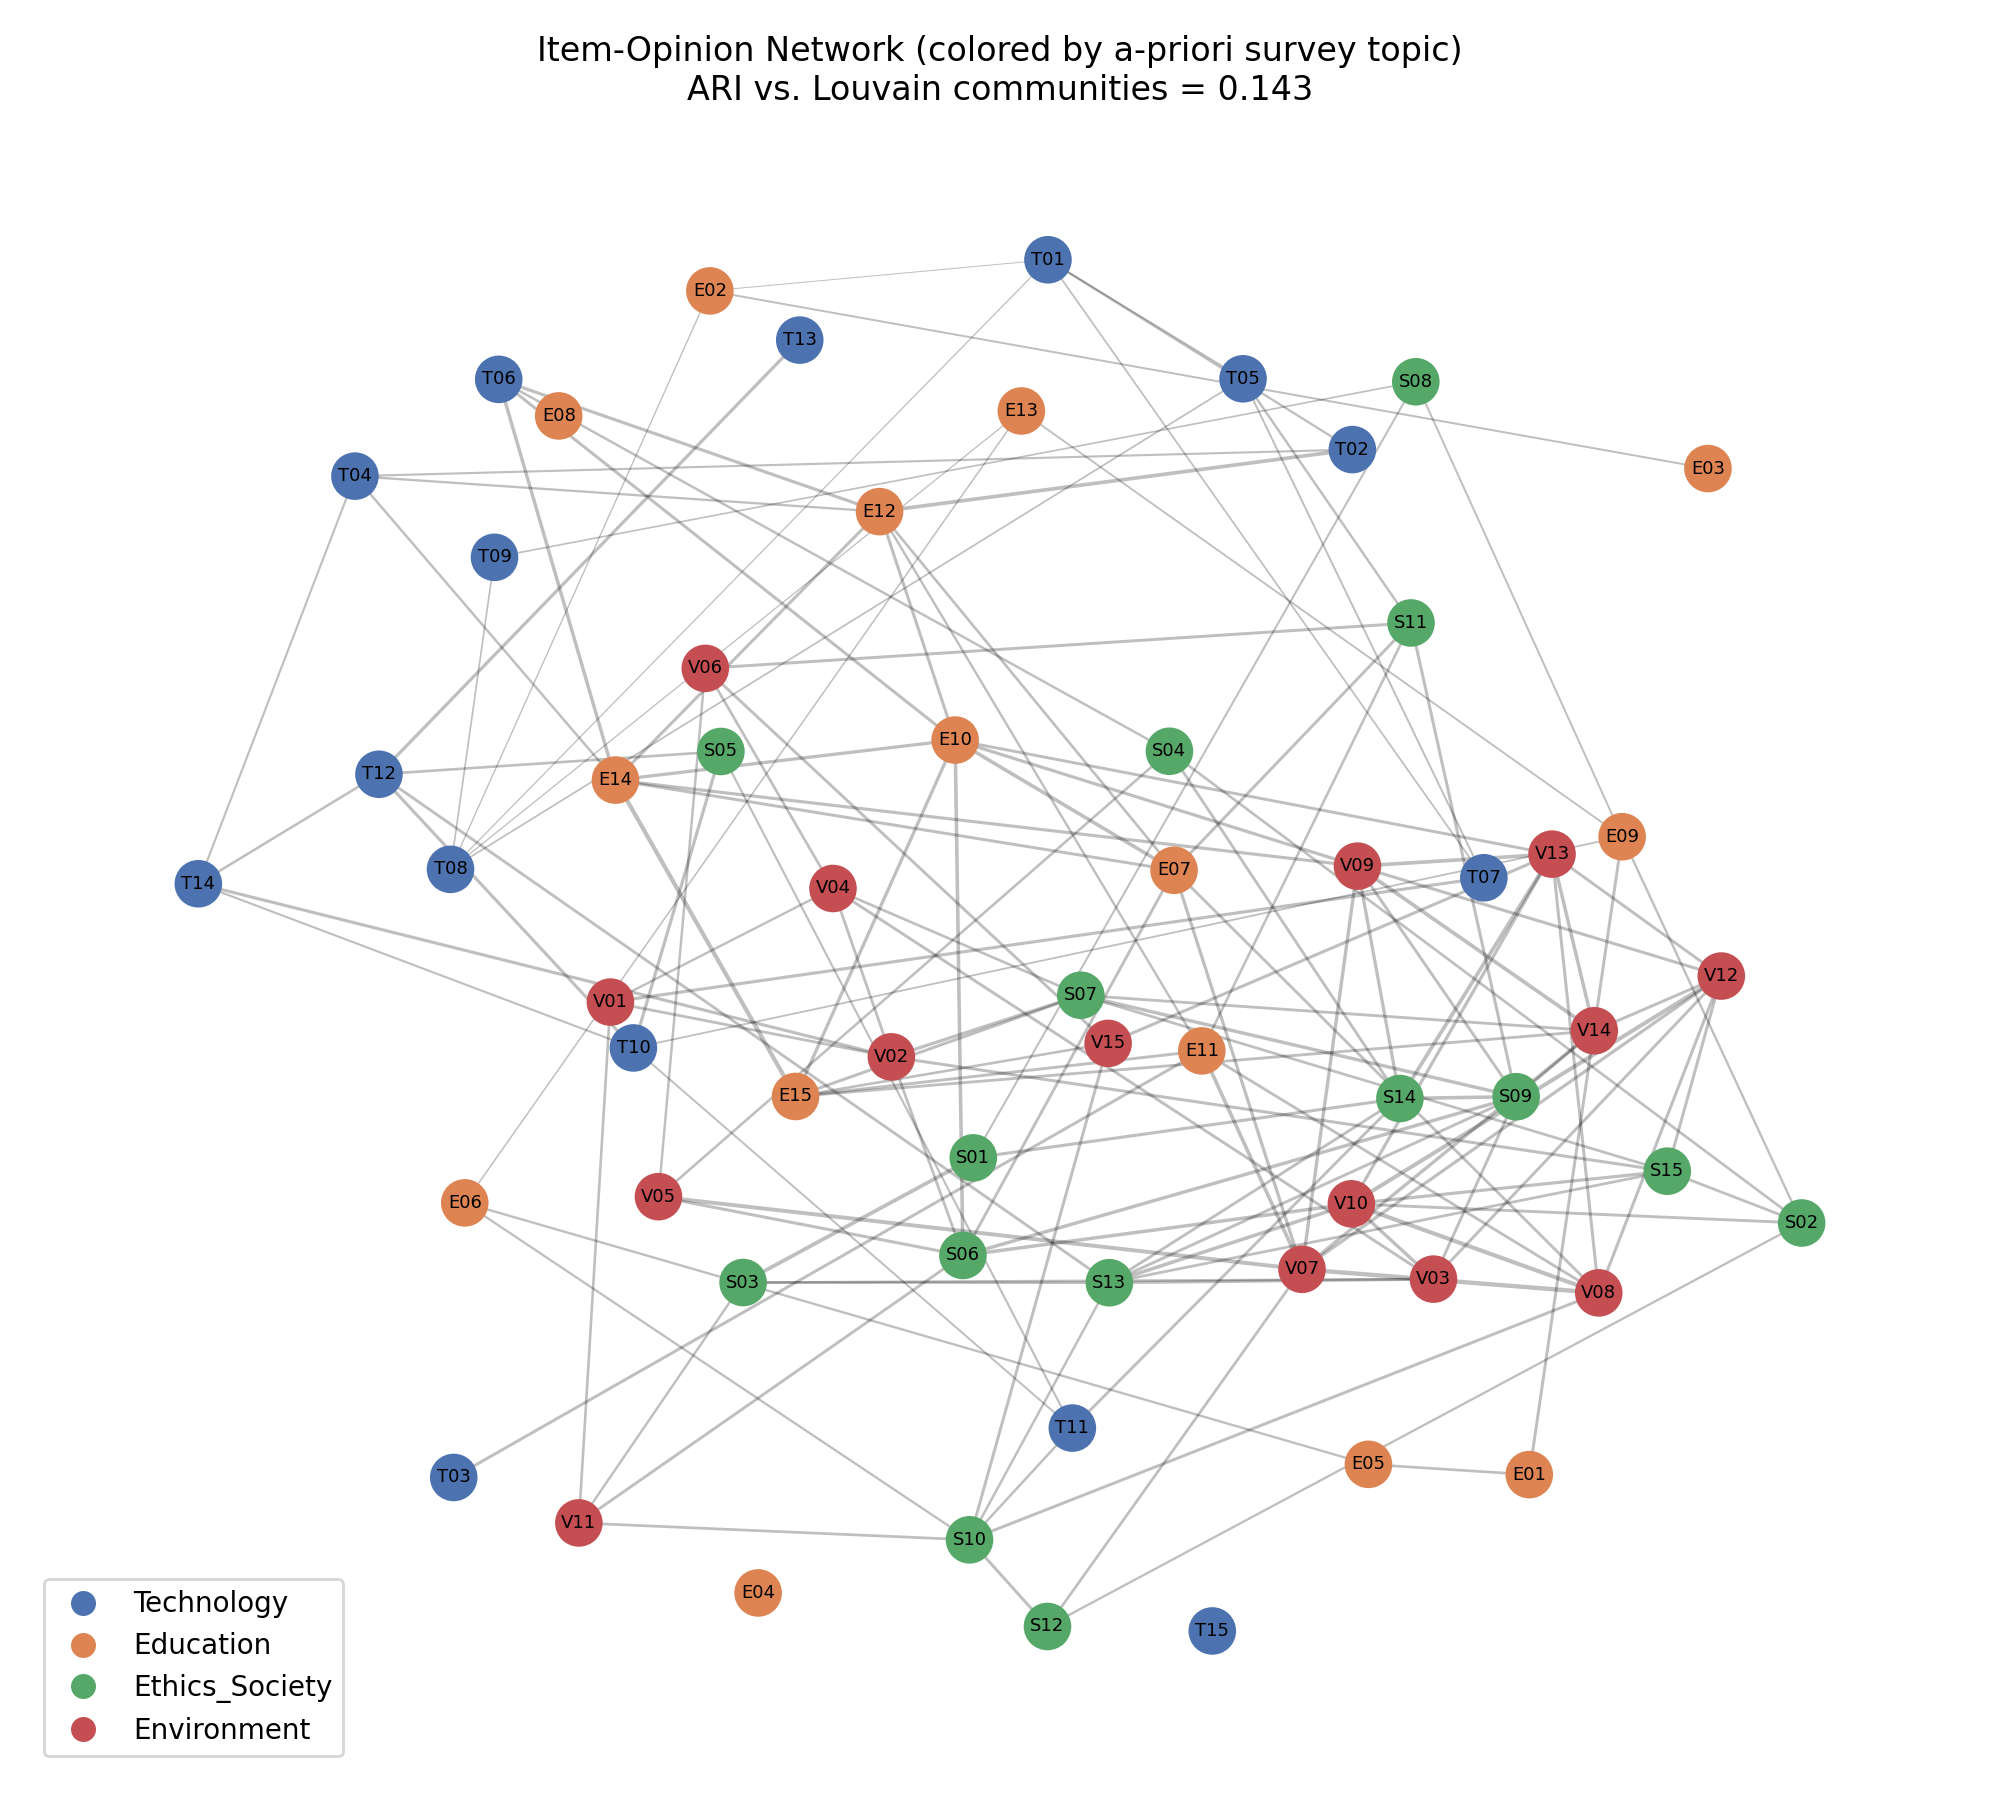
\includegraphics[width=0.75\textwidth]{../../item_network/figures/item_network_by_topic.png}
\caption{The same item-opinion network and layout as
Figure~\ref{fig:item_by_community}, but colored by the survey's
a-priori topic label instead of the discovered community. The visual
mismatch between the two colorings reflects the low ARI (0.143) between
them.}
\label{fig:item_by_topic}
\end{figure}

\begin{figure}[h]
\centering
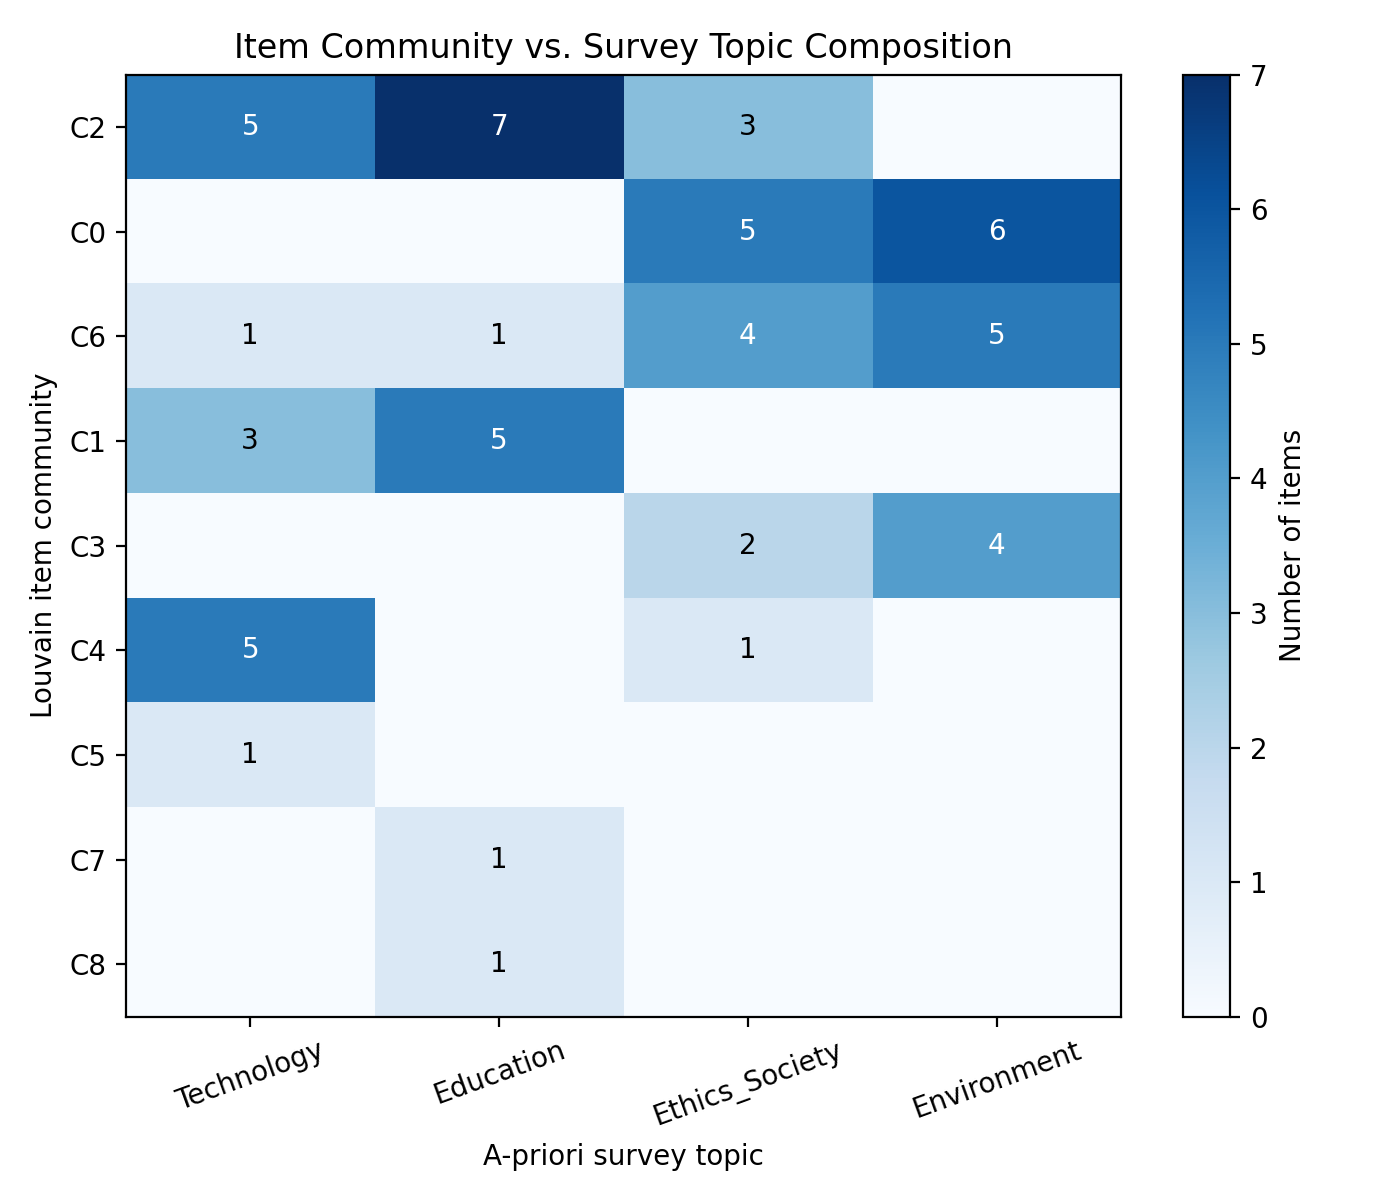
\includegraphics[width=0.7\textwidth]{../../item_network/figures/item_community_topic_heatmap.png}
\caption{Number of items from each a-priori survey topic contained in
each discovered Louvain item community. The two largest communities
each draw items from two different topics rather than one.}
\label{fig:item_heatmap}
\end{figure}

\todo{PRATHISH (Statistical Validation): insert null-model validation figures here (e.g.
histogram of null-model modularity scores with observed modularity
marked, significance test results).}

% =====================================================================
\section{Results and Discussion}
\label{sec:results}

\subsection{Person-Opinion Network (this workstream)}

The overall opinion network fragments into approximately 25 Louvain
communities at a modularity of 0.578, indicating that class opinion is
organized into many small, fine-grained groups rather than 2--3 broad
ideological camps.

Comparing topic-specific community structure to the overall network via
Adjusted Rand Index shows that \textbf{Education} (ARI = 0.181) and
\textbf{Technology} (ARI = 0.101) opinions are the strongest predictors
of a respondent's overall opinion-community membership, while
\textbf{Ethics/Society} (ARI = 0.023) and \textbf{Environment}
(ARI = 0.030) opinions are essentially uncorrelated with overall
clustering. This suggests that ethics and environmental questions attract
broad, cross-cutting agreement or disagreement that does not track the
same social groupings visible in tech/education opinions.

The bridge analysis further shows that the network's cohesion depends on
a small number of specific individuals rather than broad consensus:
respondent 81's immediate neighbors span 5 distinct communities, more
than any other node, making this respondent (and the four others in
Table~\ref{tab:bridges}) structurally critical to keeping otherwise
separate opinion groups connected.

The community opinion archetypes reveal clearly interpretable clusters:
for example, community 0 (9 members) scores well below the class average
on both Ethics/Society and Environment items -- a coherent ``skeptic''
archetype -- while community 16 (6 members) scores above average on every
topic, representing a small ``strong-consensus'' cluster.

\subsection{Item-Opinion Network (this workstream)}

The item-opinion network is noticeably less cleanly separated than the
person-opinion network: Louvain finds 9 communities at modularity
$\approx 0.43$ (versus 25 communities at modularity 0.578 for people),
and three of those nine are singleton or near-singleton items with
degree 0--1 -- individual statements that nobody's answer pattern
strongly tracks. Survey items, in other words, are more weakly and
diffusely related to one another than respondents are to each other.

More importantly, the item communities do \emph{not} reproduce the
survey's own four-topic design: ARI between Louvain item communities
and the a-priori topic labels is only 0.143. Instead of Technology,
Education, Ethics/Society, and Environment each forming their own
tight cluster, the two largest communities each blend two nominal
topics: one groups most Technology and Education items together (a
``modernization / innovation-attitude'' dimension -- how someone feels
about AI in the classroom correlates with how they feel about AI in
society generally), while another groups most Ethics/Society and
Environment items together (a ``collective responsibility''
dimension). This is a genuinely different axis of variation than the
survey's own category labels would suggest.

This finding lines up closely with the person-network results above.
Recall that Education and Technology opinions were the strongest
predictors of a respondent's overall community membership (ARI 0.18 and
0.10), while Ethics/Society and Environment opinions were essentially
uncorrelated with it (ARI $\approx 0.02$--$0.03$). The item-level
picture explains \emph{why}: Ethics/Society and Environment items are
exactly the ones with the highest agreement and lowest spread in the
descriptive statistics (Table~\ref{tab:topic_stats} -- means of 1.28
and 1.39 out of 2, with the smallest standard deviations of any topic).
When almost everyone agrees with an item, that item carries very little
information about how respondents differ from one another, so it
cannot drive person-level community structure even though it clusters
tightly with other similarly-high-consensus items at the item level.
Technology and Education items, by contrast, have more spread (std.\
0.99 and 1.15) and therefore more genuine disagreement to organize
people around -- consistent with them being the topics that best
predict overall person-community membership.

\todo{PRATHISH (Statistical Validation): discuss null-model validation findings here -- is the
observed community structure statistically significant compared to
random graphs of the same size/density? Does this justify $k=8$ as a
sparsification parameter?}

\subsection{Overall Synthesis}
\todo{ALL: once each subsection above is written, add 1 short paragraph
tying the three analyses together -- what does the combination of the
person-network, item-network, and statistical validation tell us about
how this class thinks, collectively?}

% =====================================================================
\section{Individual Contribution}
\label{sec:contribution}

\begin{itemize}
    \item \textbf{Shreem Shukla}: Cleaned and pre-processed the raw
    survey data (missing-value handling, dropping incomplete responses,
    Likert-to-numeric encoding); built the full person-opinion network
    construction pipeline (Pearson similarity, mutual $k$-NN graph
    construction, Louvain community detection, degree/betweenness/
    eigenvector centrality); performed the cross-topic ARI comparison,
    the opinion-bridge analysis, and the community opinion-archetype
    analysis. Wrote the Pipeline Followed section, the data-cleaning
    portion of Dataset Documentation, and this report skeleton.
    \item \textbf{Kris Jain}: Wrote up and elaborated the Dataset
    Documentation section (cleaning/encoding narrative, per-topic
    descriptive statistics, distribution plots, and a discussion of
    self-report survey bias). Designed and built the item-opinion
    network (\texttt{item\_network/build\_item\_network.py}): item-item
    Pearson correlation, mutual $k$-NN graph construction, Louvain
    community detection, and an Adjusted Rand Index comparison against
    the survey's a-priori topic labels to test whether real opinion
    structure follows the survey's own topic design. Produced the
    item-network figures and metrics table, and wrote the corresponding
    Item-Opinion Network subsections of Pipeline Followed, Analysis and
    Visualizations, and Results and Discussion.
    \item \textbf{Prathish Ghosh}: \todo{fill in -- e.g.
    "Designed and ran null-model statistical validation of network
    community structure; performed sensitivity analysis across k values;
    contributed to Results and Discussion."}
\end{itemize}

\end{document}
